% TODO section for explaining the evaluation process

In this chapter, we evaluate our implementation of the hard iron calibration presented in Chapter \ref{ch:impl}. First, we give an overview of the hardware used for evaluation. Then we take a look at the behaviour of the sensor data collection and a qualitative evaluation of the orientation filter. Finally, we will evaluate the quality of our hard iron calibration in comparison to the one of the system, the error estimation, and its performance.

\section{Hardware}

Four different devices were available for evaluation. They are listed in Table \ref{tbl:hardware}. It was important to compare the results between multiple devices since sensors and hard iron calibration algorithms vary between them. Also, we need to be sure that the performance of our implementation is good enough for real-time processing across different devices to achieve maximum compatibility.

All these devices run a fairly recent Android version and have been released during the last 5 years.

\begin{table}[h]
    \centering
    \begin{tabular}{ | l | r | r | }
    \hline
    \textbf{Name}     & \textbf{Release year} & \textbf{Android version} \\ \hline
    Google Pixel 3    & 2018 & 11 \\ \hline
    Google Pixel 2    & 2017 & 11 \\ \hline
    Samsung Galaxy S7 & 2016 & 8 \\ \hline
    LG Nexus 5X       & 2015 & 8.1 \\ \hline
    \end{tabular}
    \caption{Devices used for testing and evaluation.}
    \label{tbl:hardware}
\end{table}

Another possible test device was the Nokia 3 released in 2017 but unfortunately it does not provide uncalibrated magnetic field sensor readings. Up to this point we are not sure about the market share of devices that support uncalibrated readings. Alternatives will be discussed in Chapter \ref{ch:outlook}.

\section{Data collection}
\label{sec:eval_sensor}

The validation of the sensor data collection was a first and important step for evaluation, since all the following steps depend on it. Moreover, it was beneficial for building up intuition for the data which is used for filtering.

This experiment was carried out on all the Android test devices listed in Table \ref{tbl:hardware}. The requested sampling interval was $1$ ms.

As a first step, only the timestamps of the magnetometer readings were used to calculate the measurement interval. Since Android is not a real-time system the interval will not be constant. A histogram of the interval is shown in Figure \ref{fig:interval}. Statistics are given in Table \ref{tbl:mag_interval}.
% TODO point out that the measured sampling intervals is very different from the one requested

\begin{figure}[hbt!]
    \centering
    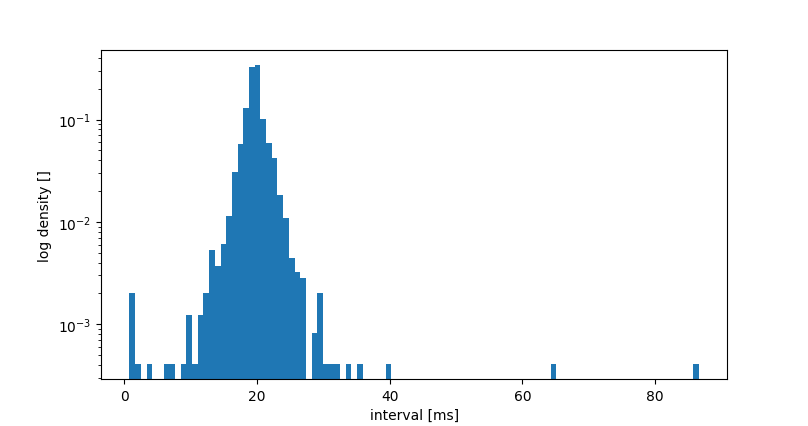
\includegraphics[width=1.0\textwidth]{figures/interval_nexus5.png}
    \caption{Histogram of the of the sampling interval for the magnetometer in the LG Nexus 5X.}
    \label{fig:interval}
\end{figure}

\begin{table}[h]
    \centering
    \begin{tabular}{ | l | r | r | r | r | r | r | r | }
    \hline
    \textbf{Device}   & \textbf{mean} & \textbf{std} & \textbf{min} & $\bm{Q_1}$ & \textbf{median} & $\bm{Q_3}$ & \textbf{max} \\ \hline
    Google Pixel 3    & 10.0 & 3.2 & 0.1 &  9.0 & 10.0 & 11.2 &  57.4 \\ \hline
    Google Pixel 2    &  9.6 & 1.6 & 0.0 &  9.2 &  9.6 &  9.9 &  63.9 \\ \hline
    Samsung Galaxy S7 & 10.0 & 2.6 & 0.3 &  9.3 & 10.0 & 10.7 & 115.5 \\ \hline
    LG Nexus 5X       & 19.7 & 2.6 & 0.8 & 19.0 & 19.7 & 20.4 &  86.5 \\ \hline
    \end{tabular}
    \caption{Statistics of the magnetometer reading interval in milliseconds.}
    \label{tbl:mag_interval}
\end{table}

Secondary, the readings of the magnetometer were displayed as a three-dimensional scatter plot to reveal the hard iron effect. For this purpose the device has been rotated in multiple directions while reading the magnetic field. Two-dimensional projections of such a three-dimensional scatter are shown in Figure \ref{fig:scatter} for the Samsung Galaxy S7.

\begin{figure}[hbt!]
    \centering
    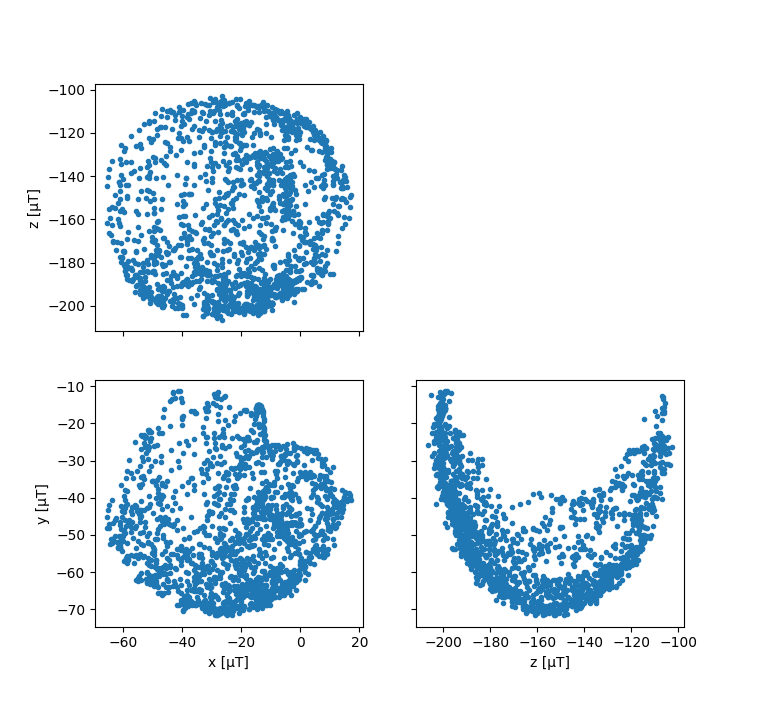
\includegraphics[width=1.0\textwidth]{figures/scatter_s7.png}
    \caption{Scatter plot of the magnetometer readings while rotating the Samsung Galaxy S7 in multiple directions.}
    \label{fig:scatter}
\end{figure}

Without the hard iron effect we would expect the center of the plots at the origin. The maximal distance from the origin should be the magnitude of the Earth's magnetic field if other environmental sources are neglectable. Measuring the horizontal orientation involves $\arctantwo(y, x)$ for a two dimensional projection of the magnetic field. As we can see in Figure \ref{fig:scatter}, without considering the hard iron effect, the estimation of the horizontal orientation would be meaningless since $(x, y, z)$ are not zero-centered.
% TODO there should be a sections for horizontal orientation estimation that we can reference here

\section{Orientation filter}
% TODO refer to impl section?

Since our hard iron calibration depends highly on the orientation estimation, it was necessary to validate the implementation and to evaluate its performance. A quantitative evaluation would require reference values for the orientation of the device for comparison. This could be achieved by tracking visual landmarks with a camera, rotating the device with a robotic arm or simulation of sensor data. Such experiments were carried out at the Department of Geodesy and Geoinformation at TU Wien in order to evaluate their Kalman-based orientation estimation.\cite{Ettlinger2018} However, using their equipment and data was not part of this thesis.

The implementation of the orientation filter required at least a qualitative evaluation to guarantee its functionality. This was carried out with an augmented reality demo application. A cube was placed at the origin of a 3D scene and the position and orientation of the camera in this scene were calculated based on the orientation of the phone in such a way, that the cube seems to be stationary in world coordinates. This approach validates the transformation between the local and global frames of reference and qualitatively evaluates the response to sensor updates.

The 3D scene is illustrated in Figure \ref{fig:cube_scene}. Pictures of the augmented cube rendered by the LG Nexus 5X are show in Figure \ref{fig:cubes}.

\begin{figure}[hbt!]
    \centering
    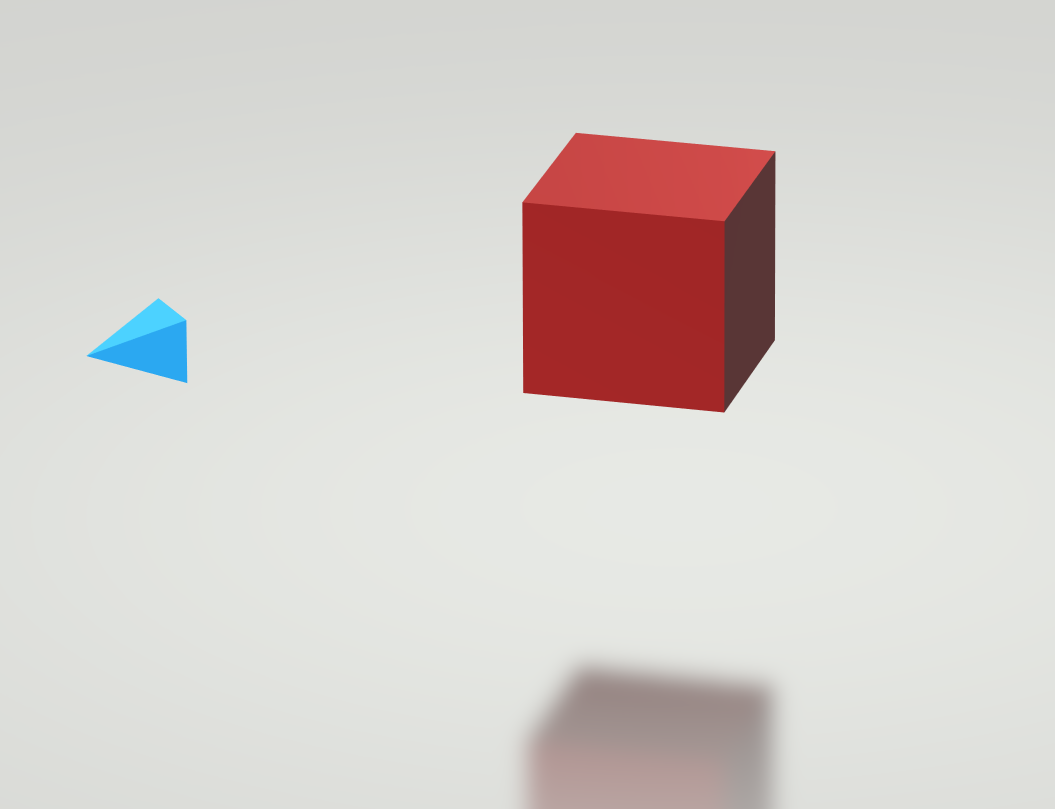
\includegraphics[width=0.6\textwidth]{figures/cube_scene.png}
    \caption{Illustration of the cube and the camera in the 3D scene.}
    \label{fig:cube_scene}
\end{figure}

\begin{figure}[hbt!]
    \centering
    \begin{subfigure}{0.3\textwidth}
        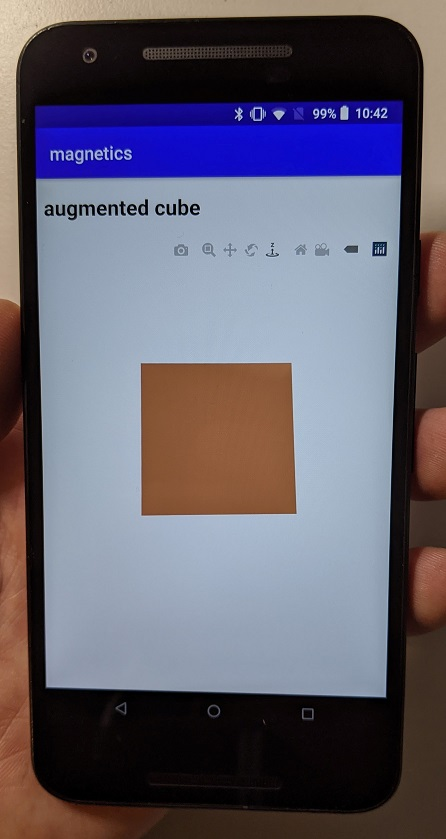
\includegraphics[height=1.5\linewidth]{figures/cube.jpg}
        %\caption{image1}
        %\label{fig:1}
    \end{subfigure}
    \begin{subfigure}{0.3\textwidth}
        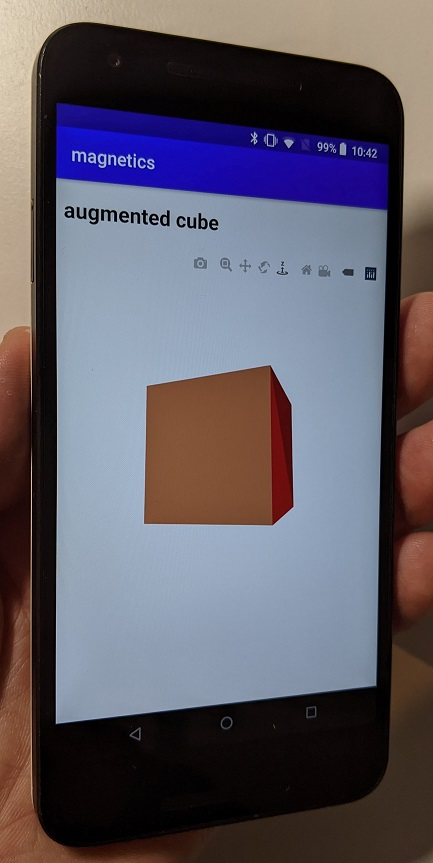
\includegraphics[height=1.5\linewidth]{figures/cube_right.jpg}
        %\caption{image1}
        %\label{fig:1}
    \end{subfigure}
    \begin{subfigure}{0.3\textwidth}
        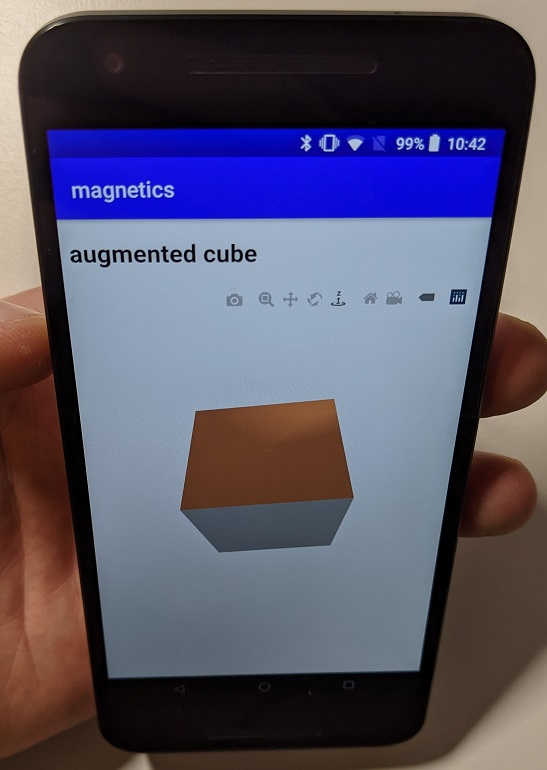
\includegraphics[height=1.5\linewidth]{figures/cube_bottom.jpg}
        %\caption{image1}
        %\label{fig:1}
    \end{subfigure}
    \caption{Pictures of the augmented cube after rotating the device.}
    \label{fig:cubes}
\end{figure}

The accelerometer and gyroscope have been down sampled to a 50 ms interval. Therefore, some delay and low refresh rate was expected. However, the experience was very positive.

The orientation filter has only a single parameter \textsc{beta}, apart from the update interval. \textsc{beta} models the reliability proportion between accelerometer and gyroscope measurements. This parameter has to be chosen carefully and in the best case individually for each sensor composition or smartphone model, since quality of the estimates depends highly upon that. Choosing one parameter across multiple devices might result in low accuracy or biased estimated.

Our demo application can be used to hand-tune \textsc{beta} for a given device. One could chose a parameter to start with and test it in the application. By observing the performance one might decide that the parameter is not optimal and change it. Following this process iteratively until the results are satisfying will lead to an optimized value for \textsc{beta}.

\section{Hard iron calibration}
% visualize particle cloud over time

% left over oscillations might be due to latency in orientation estimation or soft iron effects (read somewhere that magnetization only takes ns so that might be bs)
%  - rather small ~1µT so not that important for orientation but never the less interesting

A test track was set up in order to evaluate our hard iron calibration. It is illustrated in Figure \ref{fig:eval_scenario}. Visual landmarks were placed at each turning point as a spatial reference for the collected sensor data across different devices. The track had a total length of approximately 24 meters with 4 turns and a total horizontal rotation angle of approximately 540 degrees. A button in the test application, called \textsc{tick} (see Figure \ref{fig:app}), was used to mark the passing of each landmark.

\begin{figure}[H]
    \centering
    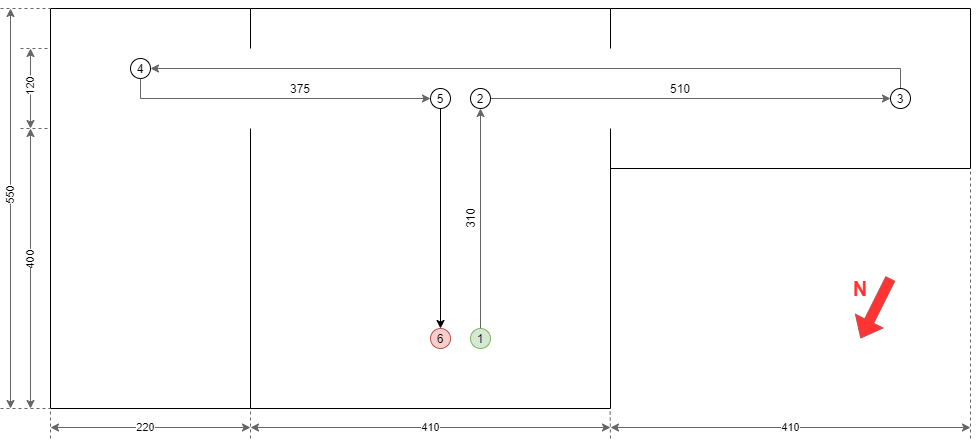
\includegraphics[width=1.0\textwidth]{figures/scenario.png}
    \caption{Illustration of the test scenario for the hard iron calibration.}
    \label{fig:eval_scenario}
\end{figure}

Each test run was a sequence of three different phases. In the first phase the test device was placed on a table. Thereby, the orientation estimation would initialize in the same way across different test runs. Then a magnet was used in order to manipulate the hard iron effect of the test device. The second phase started by pressing the \textsc{tick} button in the application, followed by walking the test track. The average walking speed was approximately 1 m/s. The third phase started with a last press of the \textsc{tick} button at landmark 6. Then the test device was rotated in multiple directions on the same position. With the third and last phase we collected a large amount of reference data for an optimal magnetometer calibration.

The test application would be started with the button \textsc{start rec} (see Figure \ref{fig:app}), an abbreviation for ``start recording''. By pressing this button, our application starts to record all the incoming data from the sensors. Our \textsc{tick} button is also treated like a sensor in this case. Each sensor reading is then stored in a file, along with its timestamp. The recorded data was later used to simulate the sensor input and to evaluate the output of our filter. Table \ref{tbl:eval_params} contains the parameters of our filter used during the simulation.

\begin{table}[H]
    \centering
    \begin{tabular}{ | l | r | }
    \hline
    \textbf{Parameter}              & \textbf{Value} \\ \hline
    \textsc{seed}                   & random \\ \hline
    \textsc{population}             & $10^5$ \\ \hline
    \textsc{deltaTime}              & 50 ms \\ \hline
    \textsc{initialVariance}        & $(100\ \mu T)^2$ \\ \hline
    \textsc{driftRate}              & $1.0$ \\ \hline
    \textsc{predictionVariance}     & $(5\ \mu T)^2$ \\ \hline
    \textsc{minimalRotation}        & $0.1$ \\ \hline
    \textsc{resamplingRate}         & $0.01$ \\ \hline
    \end{tabular}
    \caption{Chosen parameters for the simulation.}
    \label{tbl:eval_params}
\end{table}

The data of the third phase of our test runs was used to estimate an independent reference for the hard iron calibration. The chosen estimator was a least squares fit for a sphere with an unknown origin and radius.\cite{Jekel2016} 

Figures \ref{fig:eval_simulation_pixel3}, \ref{fig:eval_simulation_pixel2}, \ref{fig:eval_simulation_s7}, and \ref{fig:eval_simulation_nexus5x} show the \textcolor{blue}{estimated hard iron bias and error} of our particle filter over time compared to the \textcolor{red}{least squares} estimate. The vertical lines represent the time when a landmark was passed on the test track.

Tables \ref{tbl:eval_simulation_pixel3}, \ref{tbl:eval_simulation_pixel2}, \ref{tbl:eval_simulation_s7}, and \ref{tbl:eval_simulation_nexus5x} contain the values of the estimated hard iron bias and error across different methods after passing the landmarks on the test track. \textsc{PF} is our real-time particle filter estimate, \textsc{SYS} is the system's estimate, and \textsc{LS} the post processed least squares estimate. Phase 2.x denotes passing the landmark x on the test track. Phase 3 denotes the end of the experiment after rotating the phone in multiple directions.

In all our test cases the \gls{os} was not able to calibrate the hard iron effect while walking on the test track. Only in the last phase of the experiment, when the device was rotated in multiple directions. The estimates of the systems were very close to the least squares estimates.

Figure \ref{fig:eval_simulation_pixel3} and Table \ref{tbl:eval_simulation_pixel3} show the convergence of the hard iron estimation for the Google Pixel 3. Our particle filter calibration performed very well, but picked up a bias on the z-axis after landmark 4 (phase 2.4 in the table). During the calibration phase at the end of the experiment there was a bias on the x-axis.

\begin{figure}[H]
    \centering
    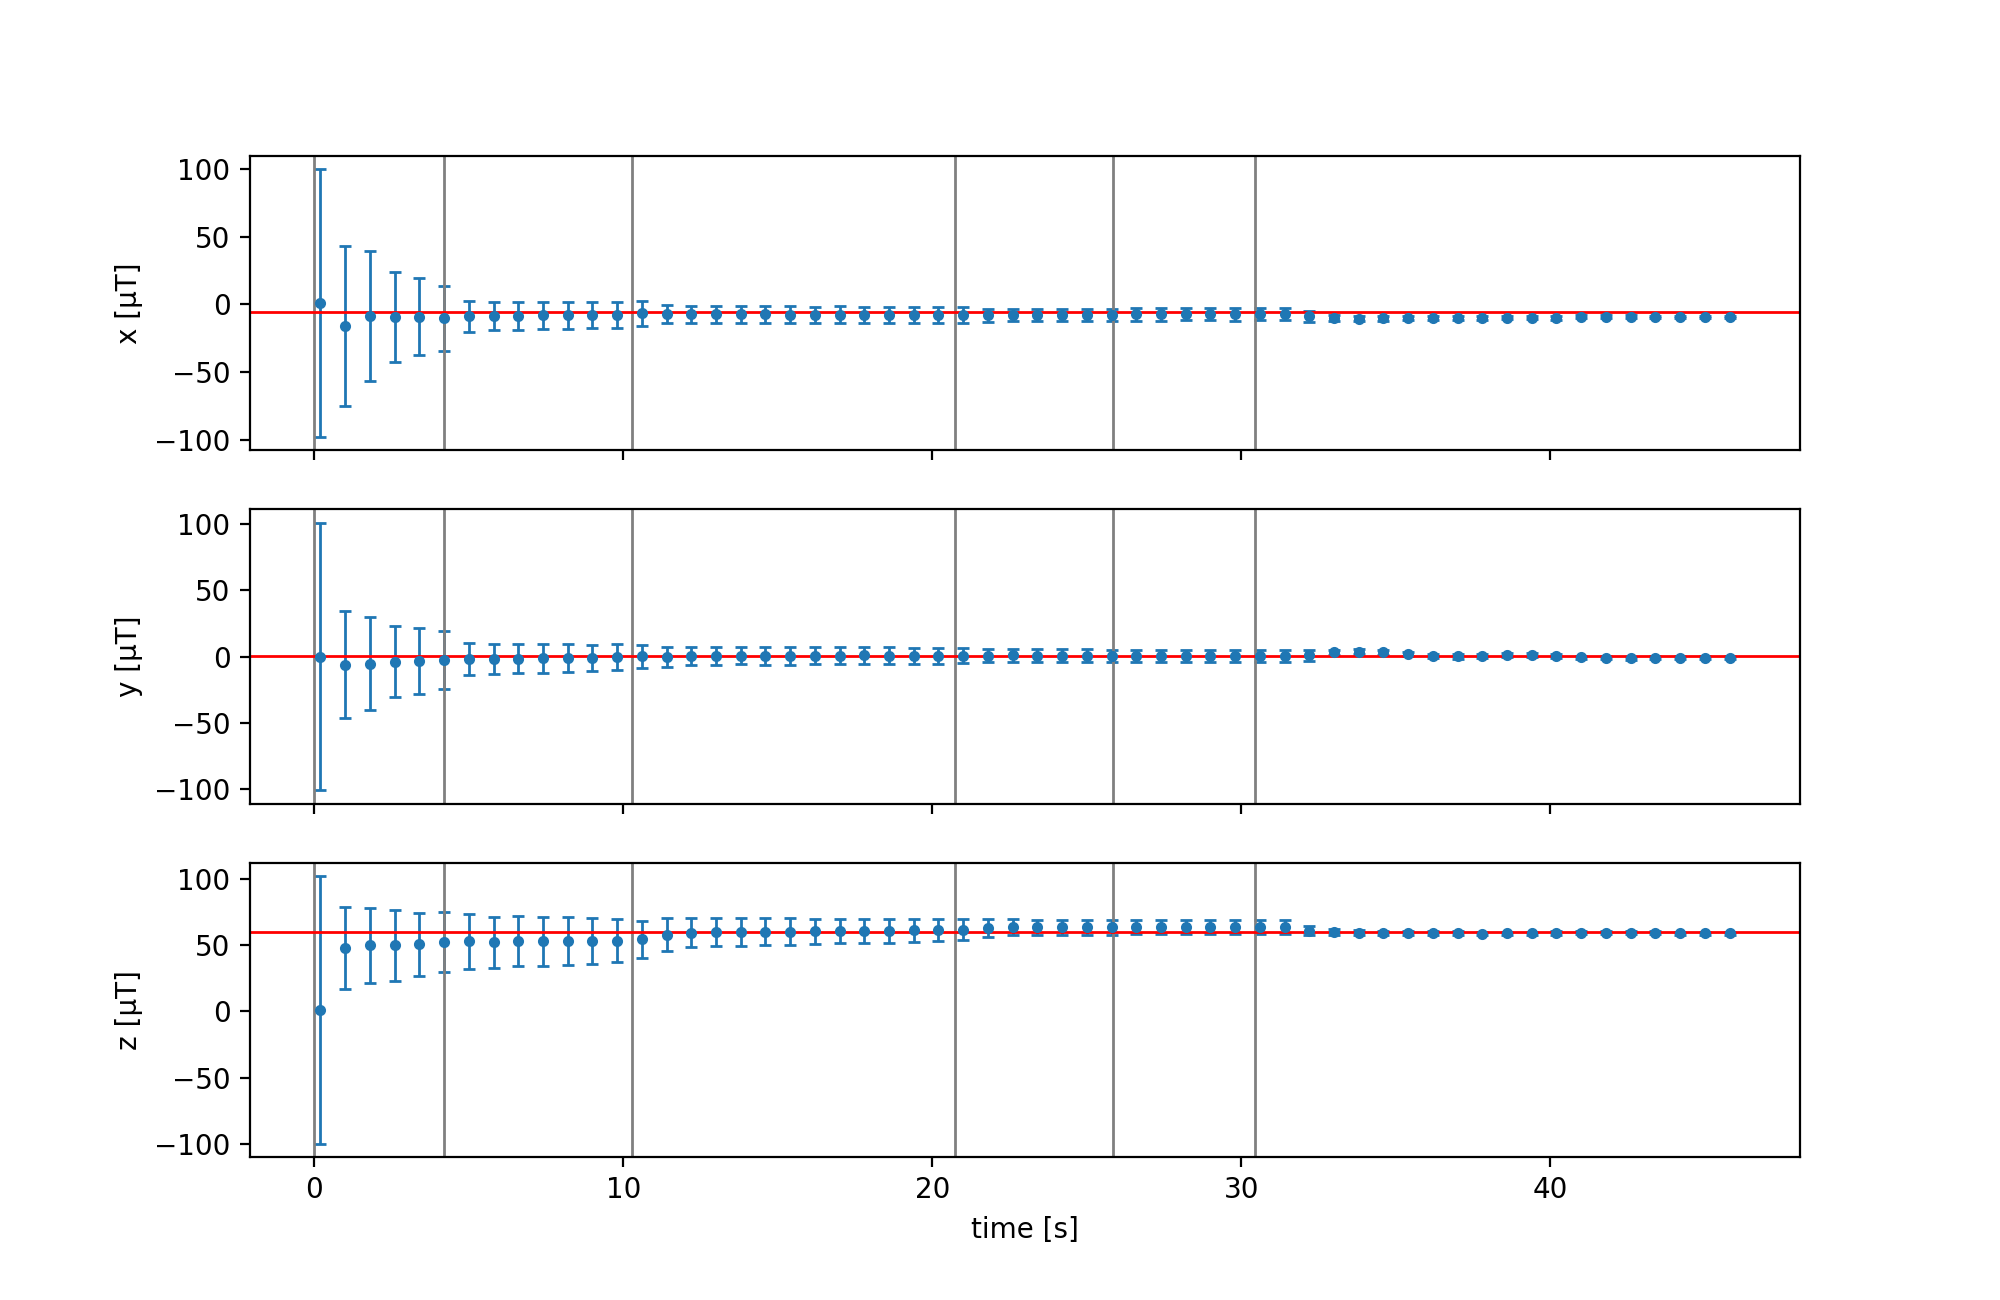
\includegraphics[width=1.0\textwidth]{figures/convergence_pixel3.png}
    \caption{Estimated hard iron bias and error over time on the Google Pixel 3.}
    \label{fig:eval_simulation_pixel3}
\end{figure}

\begin{table}[H]
    \centering
    \resizebox{\columnwidth}{!}{
    \begin{tabular}{ | l | l | r | r | r | r | r | r | r | }
    \hline
    \textbf{Method} & \textbf{Axis} & \textbf{Phase 2.1} & \textbf{Phase 2.2} & \textbf{Phase 2.3} & \textbf{Phase 2.4} & \textbf{Phase 2.5} & \textbf{Phase 2.6} & \textbf{Phase 3} \\ \hline
    PF  & X & $-0.5\pm100.5$ & $-9.3\pm24.0$ & $-5.8\pm7.2$ & $-5.3\pm4.6$ & $-5.3\pm3.9$ & $-4.9\pm3.7$ & $-8.4\pm1.1$ \\ \hline
    SYS &   & $1.0$ & $1.0$ & $1.0$ & $1.0$ & $1.0$ & $1.0$ & $-6.4$ \\ \hline
    LS  &   & & & & & & & $-5.4$ \\ \hline
    PF  & Y & $-0.6\pm100.4$ & $-3.7\pm21.6$ & $-3.3\pm8.8$ & $-2.4\pm5.0$ & $-2.3\pm4.1$ & $-2.4\pm4.0$ & $-0.9\pm1.1$ \\ \hline
    SYS &   & $32.6$ & $32.6$ & $32.6$ & $32.6$ & $32.6$ & $32.6$ & $1.3$ \\ \hline
    LS  &   & & & & & & & $0.3$ \\ \hline
    PF  & Z & $1.2\pm100.8$ & $52.1\pm22.5$ & $53.4\pm15.4$ & $61.5\pm8.1$ & $63.3\pm5.8$ & $63.7\pm5.4$ & $58.9\pm1.1$ \\ \hline
    SYS &   & $8.4$ & $8.4$ & $8.4$ & $8.4$ & $8.4$ & $8.4$ & $59.4$ \\ \hline
    LS  &   & & & & & & & $60.1$ \\ \hline
    \end{tabular}
    }
    \caption{Estimated hard iron bias in $\mu T$ with different methods on the Google Pixel 3.}
    \label{tbl:eval_simulation_pixel3}
\end{table}

Figure \ref{fig:eval_simulation_pixel2} and Table \ref{tbl:eval_simulation_pixel2} show the convergence of the hard iron estimation for the Google Pixel 2. Our particle filter calibration looks unbiased until landmark 6 (phase 2.6 in the table) but picked up a bias during the calibration phase at the end. Here we got a small bias for the x- and y-axis.

\begin{figure}[H]
    \centering
    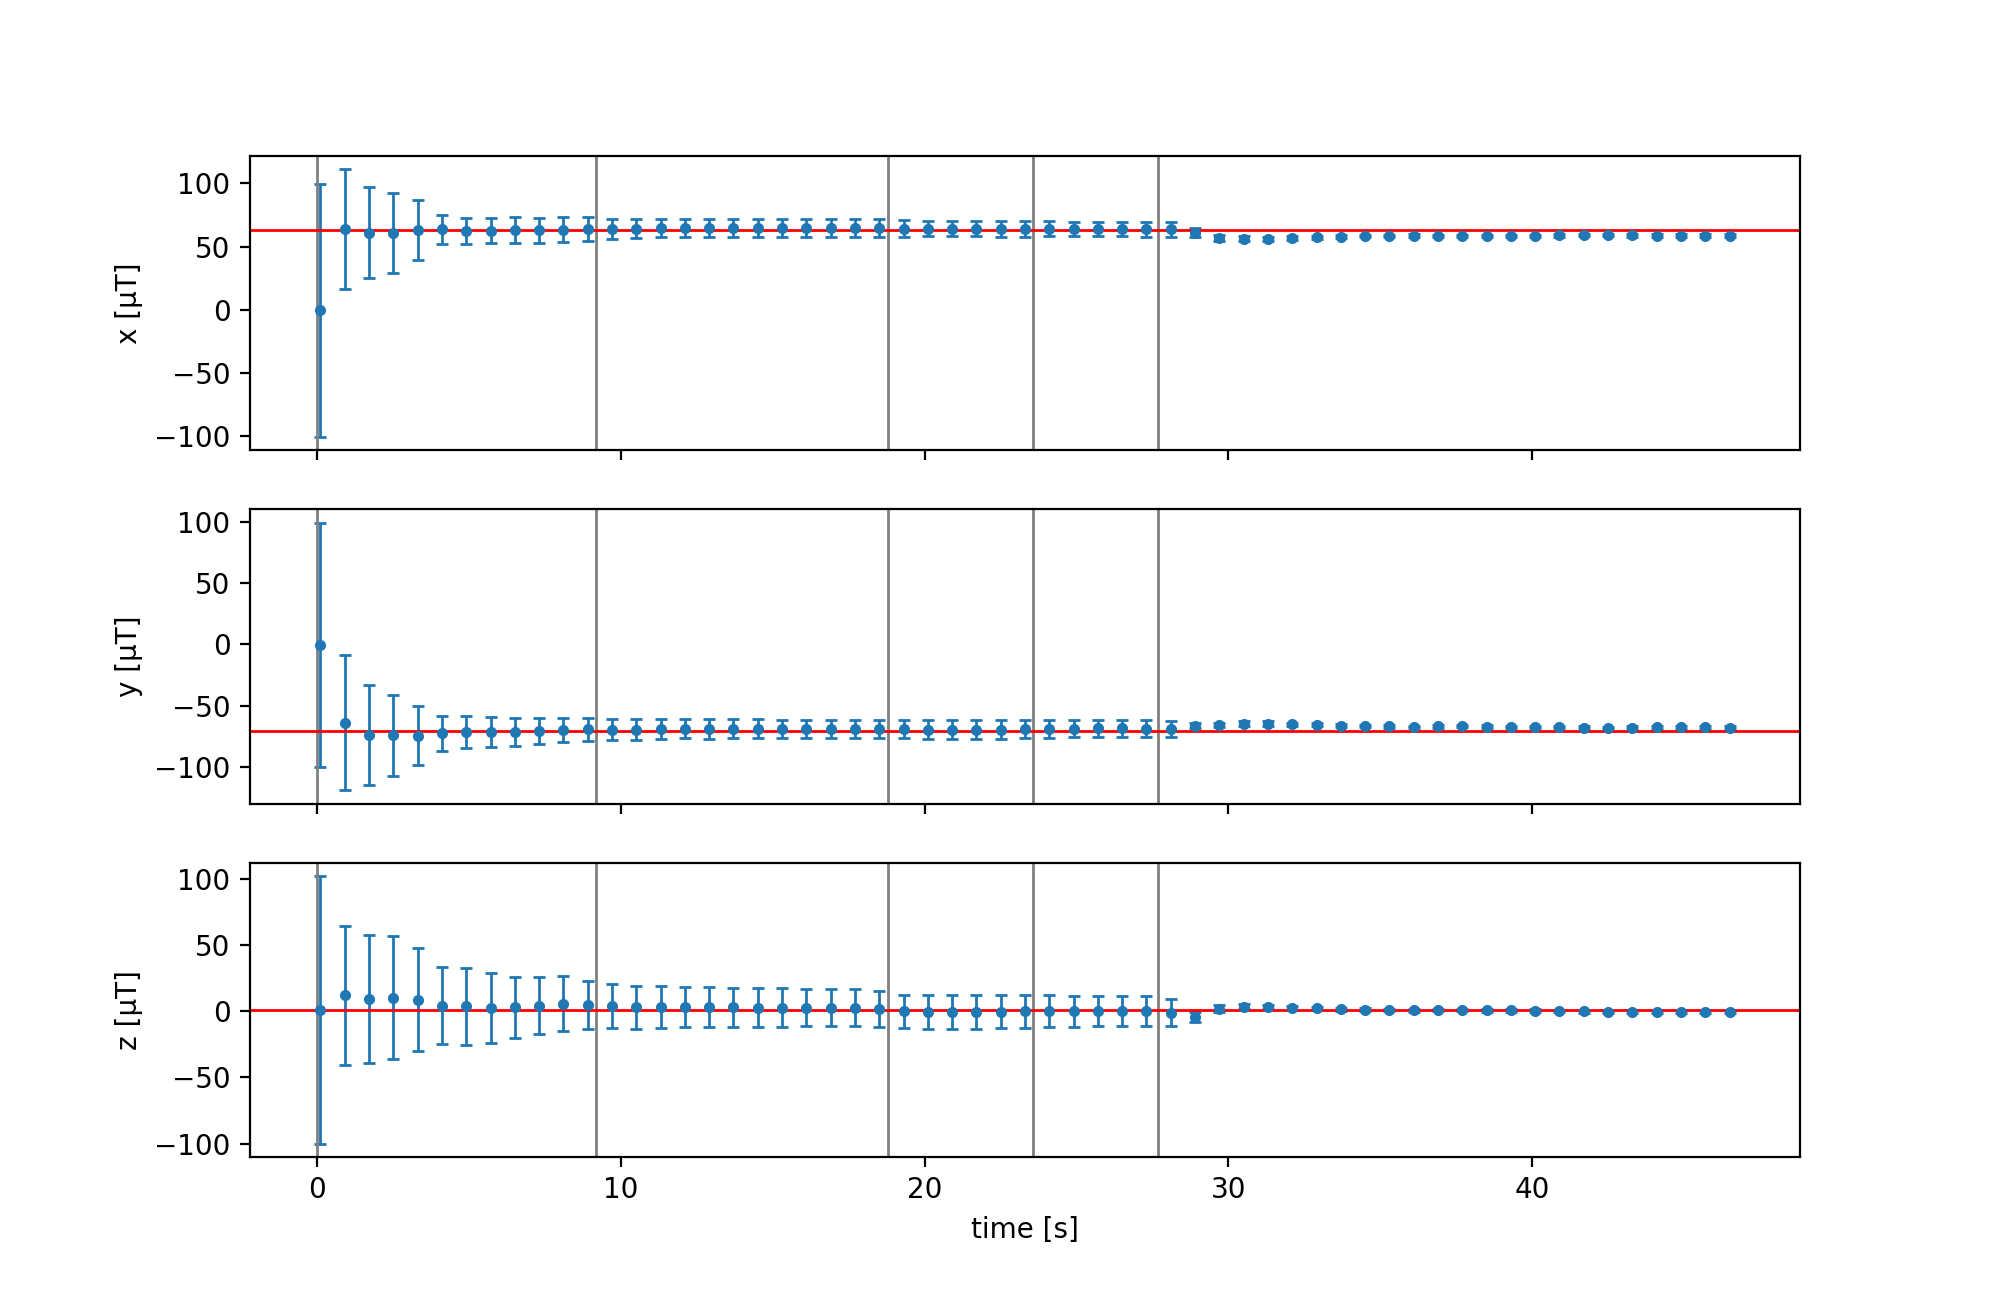
\includegraphics[width=1.0\textwidth]{figures/convergence_pixel2.png}
    \caption{Estimated hard iron bias and error over time on the Google Pixel 2.}
    \label{fig:eval_simulation_pixel2}
\end{figure}

\begin{table}[H]
    \centering
    \resizebox{\columnwidth}{!}{
    \begin{tabular}{ | l | l | r | r | r | r | r | r | r | }
    \hline
    \textbf{Method} & \textbf{Axis} & \textbf{Phase 2.1} & \textbf{Phase 2.2} & \textbf{Phase 2.3} & \textbf{Phase 2.4} & \textbf{Phase 2.5} & \textbf{Phase 2.6} & \textbf{Phase 3} \\ \hline
    PF  & X & $1.4\pm99.7$ & $62.3\pm9.1$ & $63.4\pm6.7$ & $62.7\pm5.1$ & $62.6\pm4.7$ & $59.8\pm1.7$ & $58.7\pm1.0$ \\ \hline
    SYS &   & $63.6$ & $63.6$ & $63.6$ & $63.6$ & $63.6$ & $63.6$ & $62.0$ \\ \hline
    LS  &   & & & & & & & $63.3$ \\ \hline
    PF  & Y & $0.9\pm100.1$ & $-68.7\pm11.4$ & $-70.0\pm7.6$ & $-69.1\pm6.2$ & $-68.8\pm5.8$ & $-64.2\pm1.9$ & $-67.9\pm1.0$ \\ \hline
    SYS &   & $-45.4$ & $-45.4$ & $-45.4$ & $-45.4$ & $-45.4$ & $-45.4$ & $-71.5$ \\ \hline
    LS  &   & & & & & & & $-71.2$ \\ \hline
    PF  & Z & $1.1\pm99.9$ & $1.4\pm17.7$ & $-1.2\pm11.7$ & $-0.5\pm9.2$ & $-0.0\pm8.2$ & $-3.1\pm1.6$ & $-0.2\pm1.0$ \\ \hline
    SYS &   & $-27.4$ & $-27.4$ & $-27.4$ & $-27.4$ & $-27.4$ & $-27.4$ & $-0.6$ \\ \hline
    LS  &   & & & & & & & $0.7$ \\ \hline
    \end{tabular}
    }
    \caption{Estimated hard iron bias in $\mu T$ with different methods on the Google Pixel 2.}
    \label{tbl:eval_simulation_pixel2}
\end{table}

Figure \ref{fig:eval_simulation_s7} and Table \ref{tbl:eval_simulation_s7} show the convergence of the hard iron estimation for the Samsung Galaxy S7. The hard iron effect of the z-axis was about 150 $\mu$T and therefore quite challenging. The filter would not initialize a lot of particles in close proximity since the \textsc{initialVariance} is just $(100\ \mu T)^2$. The y-axis picked up a bias most likely due to the same reason as the z-axis. During calibration phase the accuracy increases but a small bias remained on the x- and y-axis.

\begin{figure}[H]
    \centering
    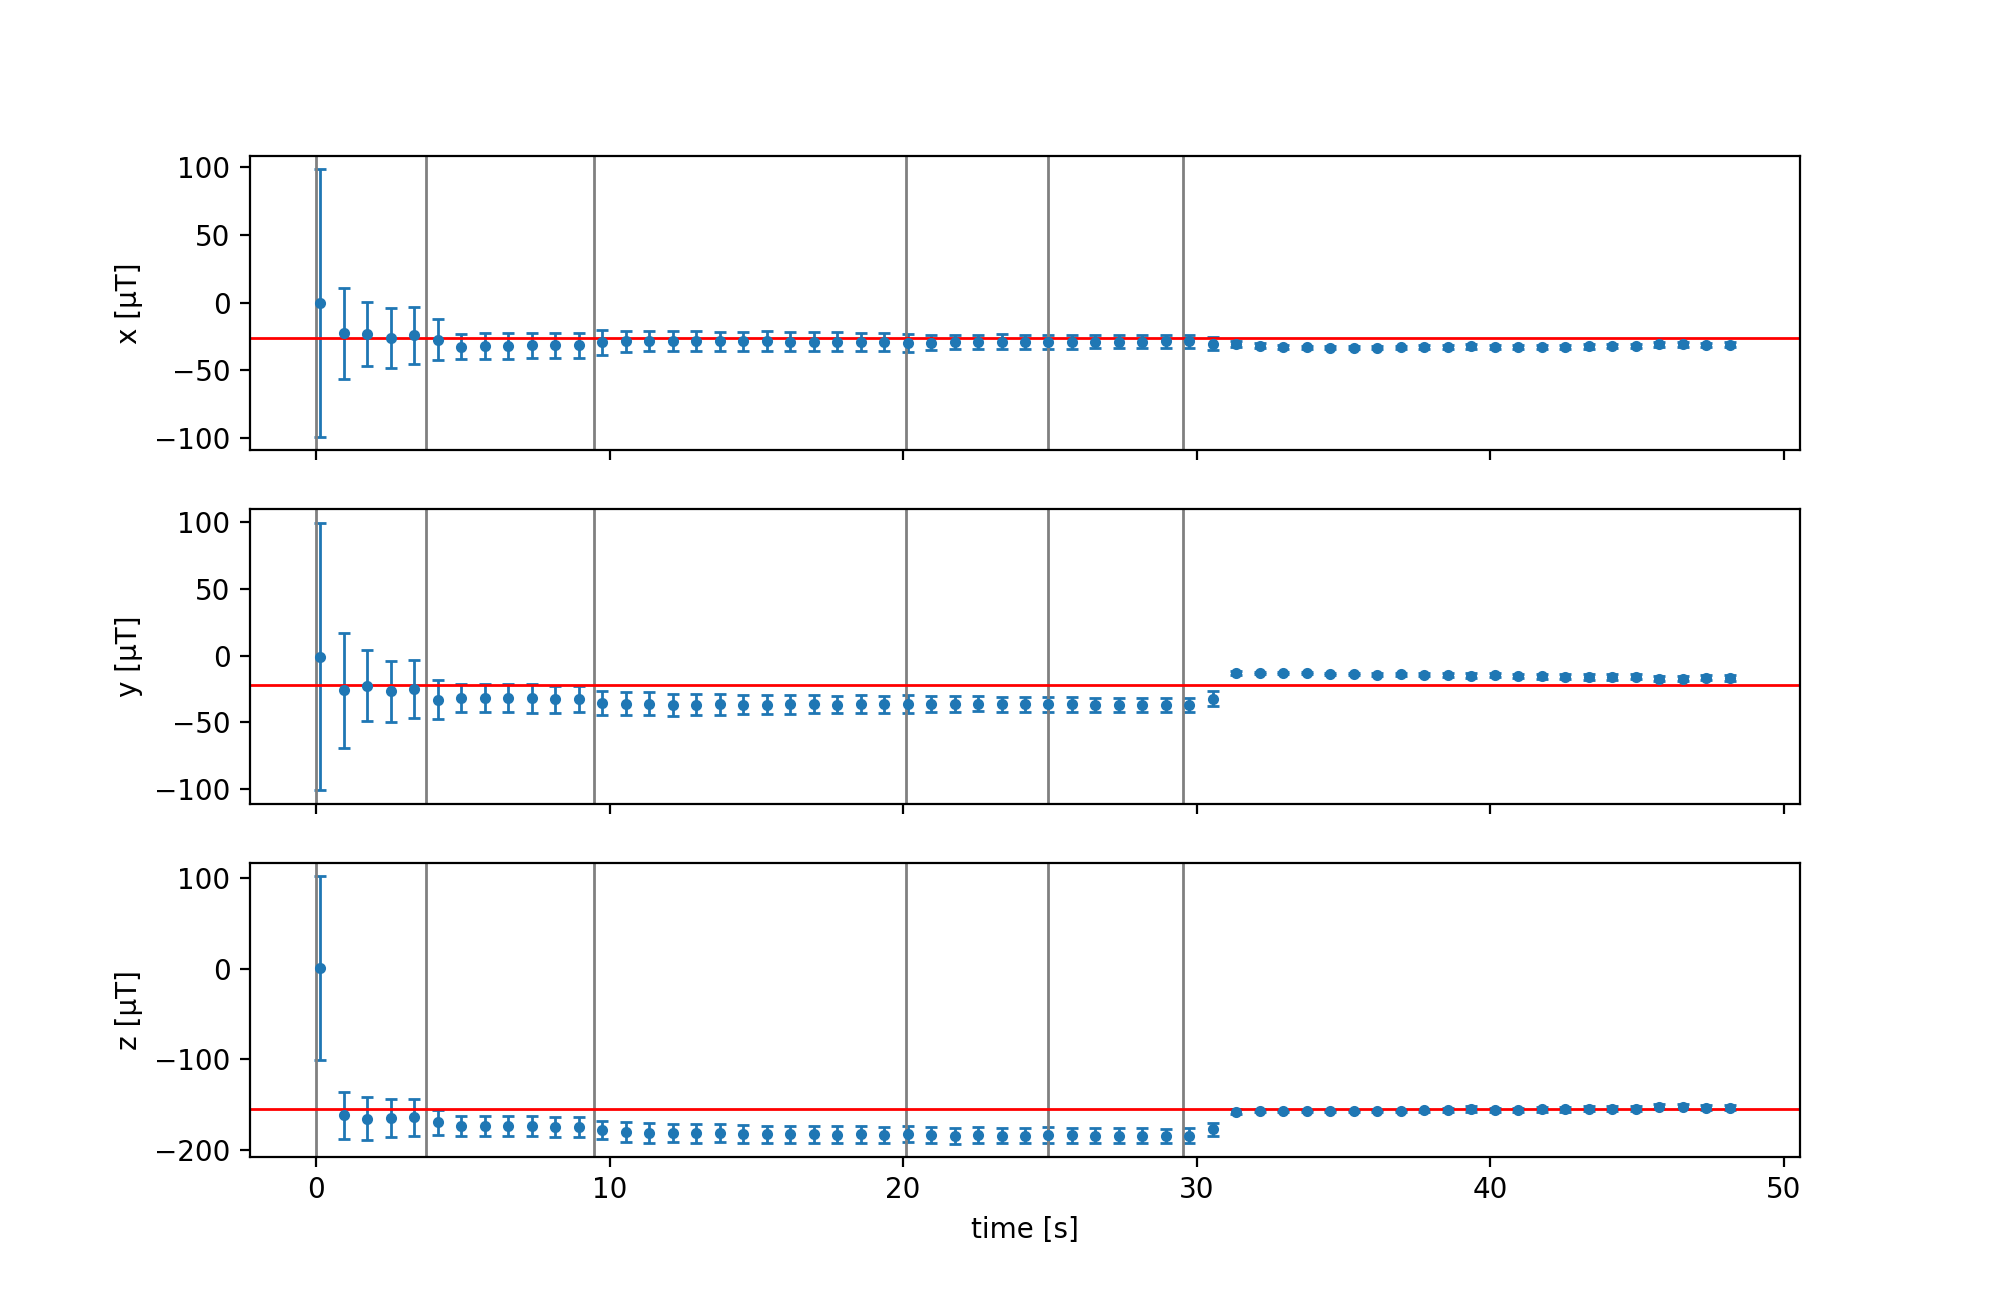
\includegraphics[width=1.0\textwidth]{figures/convergence_s7.png}
    \caption{Estimated hard iron bias and error over time on the Samsung Galaxy S7.}
    \label{fig:eval_simulation_s7}
\end{figure}

\begin{table}[H]
    \centering
    \resizebox{\columnwidth}{!}{
    \begin{tabular}{ | l | l | r | r | r | r | r | r | r | }
    \hline
    \textbf{Method} & \textbf{Axis} & \textbf{Phase 2.1} & \textbf{Phase 2.2} & \textbf{Phase 2.3} & \textbf{Phase 2.4} & \textbf{Phase 2.5} & \textbf{Phase 2.6} & \textbf{Phase 3} \\ \hline
    PF  & X & $1.1\pm100.0$ & $-20.9\pm17.2$ & $-24.1\pm7.0$ & $-24.9\pm5.5$ & $-25.8\pm4.4$ & $-26.1\pm4.2$ & $-27.2\pm1.1$ \\ \hline
    SYS &   & $0.0$ & $0.0$ & $0.0$ & $0.0$ & $0.0$ & $0.0$ & $-25.6$ \\ \hline
    LS  &   & & & & & & & $-26.1$ \\ \hline
    PF  & Y & $1.8\pm100.2$ & $-27.0\pm19.8$ & $-32.4\pm7.6$ & $-31.9\pm4.5$ & $-32.0\pm3.3$ & $-32.1\pm3.2$ & $-20.3\pm1.1$ \\ \hline
    SYS &   & $0.0$ & $0.0$ & $0.0$ & $0.0$ & $0.0$ & $0.0$ & $-23.6$ \\ \hline
    LS  &   & & & & & & & $-21.9$ \\ \hline
    PF  & Z & $0.9\pm99.9$ & $-163.8\pm16.7$ & $-167.7\pm8.9$ & $-169.8\pm6.4$ & $-170.7\pm5.1$ & $-171.1\pm4.9$ & $-154.9\pm1.2$ \\ \hline
    SYS &   & $0.0$ & $0.0$ & $0.0$ & $0.0$ & $0.0$ & $0.0$ & $-154.8$ \\ \hline
    LS  &   & & & & & & & $-154.6$ \\ \hline
    \end{tabular}
    }
    \caption{Estimated hard iron bias in $\mu T$ with different methods on the Samsung Galaxy S7.}
    \label{tbl:eval_simulation_s7}
\end{table}

Figure \ref{fig:eval_simulation_nexus5x} and Table \ref{tbl:eval_simulation_nexus5x} show the convergence of the hard iron estimation for the LG Nexus 5X. Our calibration performed reasonably well and remained within $\pm 1 \sigma$ until calibration phase. Our particle filter seemed to pick up oscillations from the rotations of the devices. This might be due to a bias in the orientation estimation. \textsc{beta} might not have been chosen optimal in this case.

\begin{figure}[H]
    \centering
    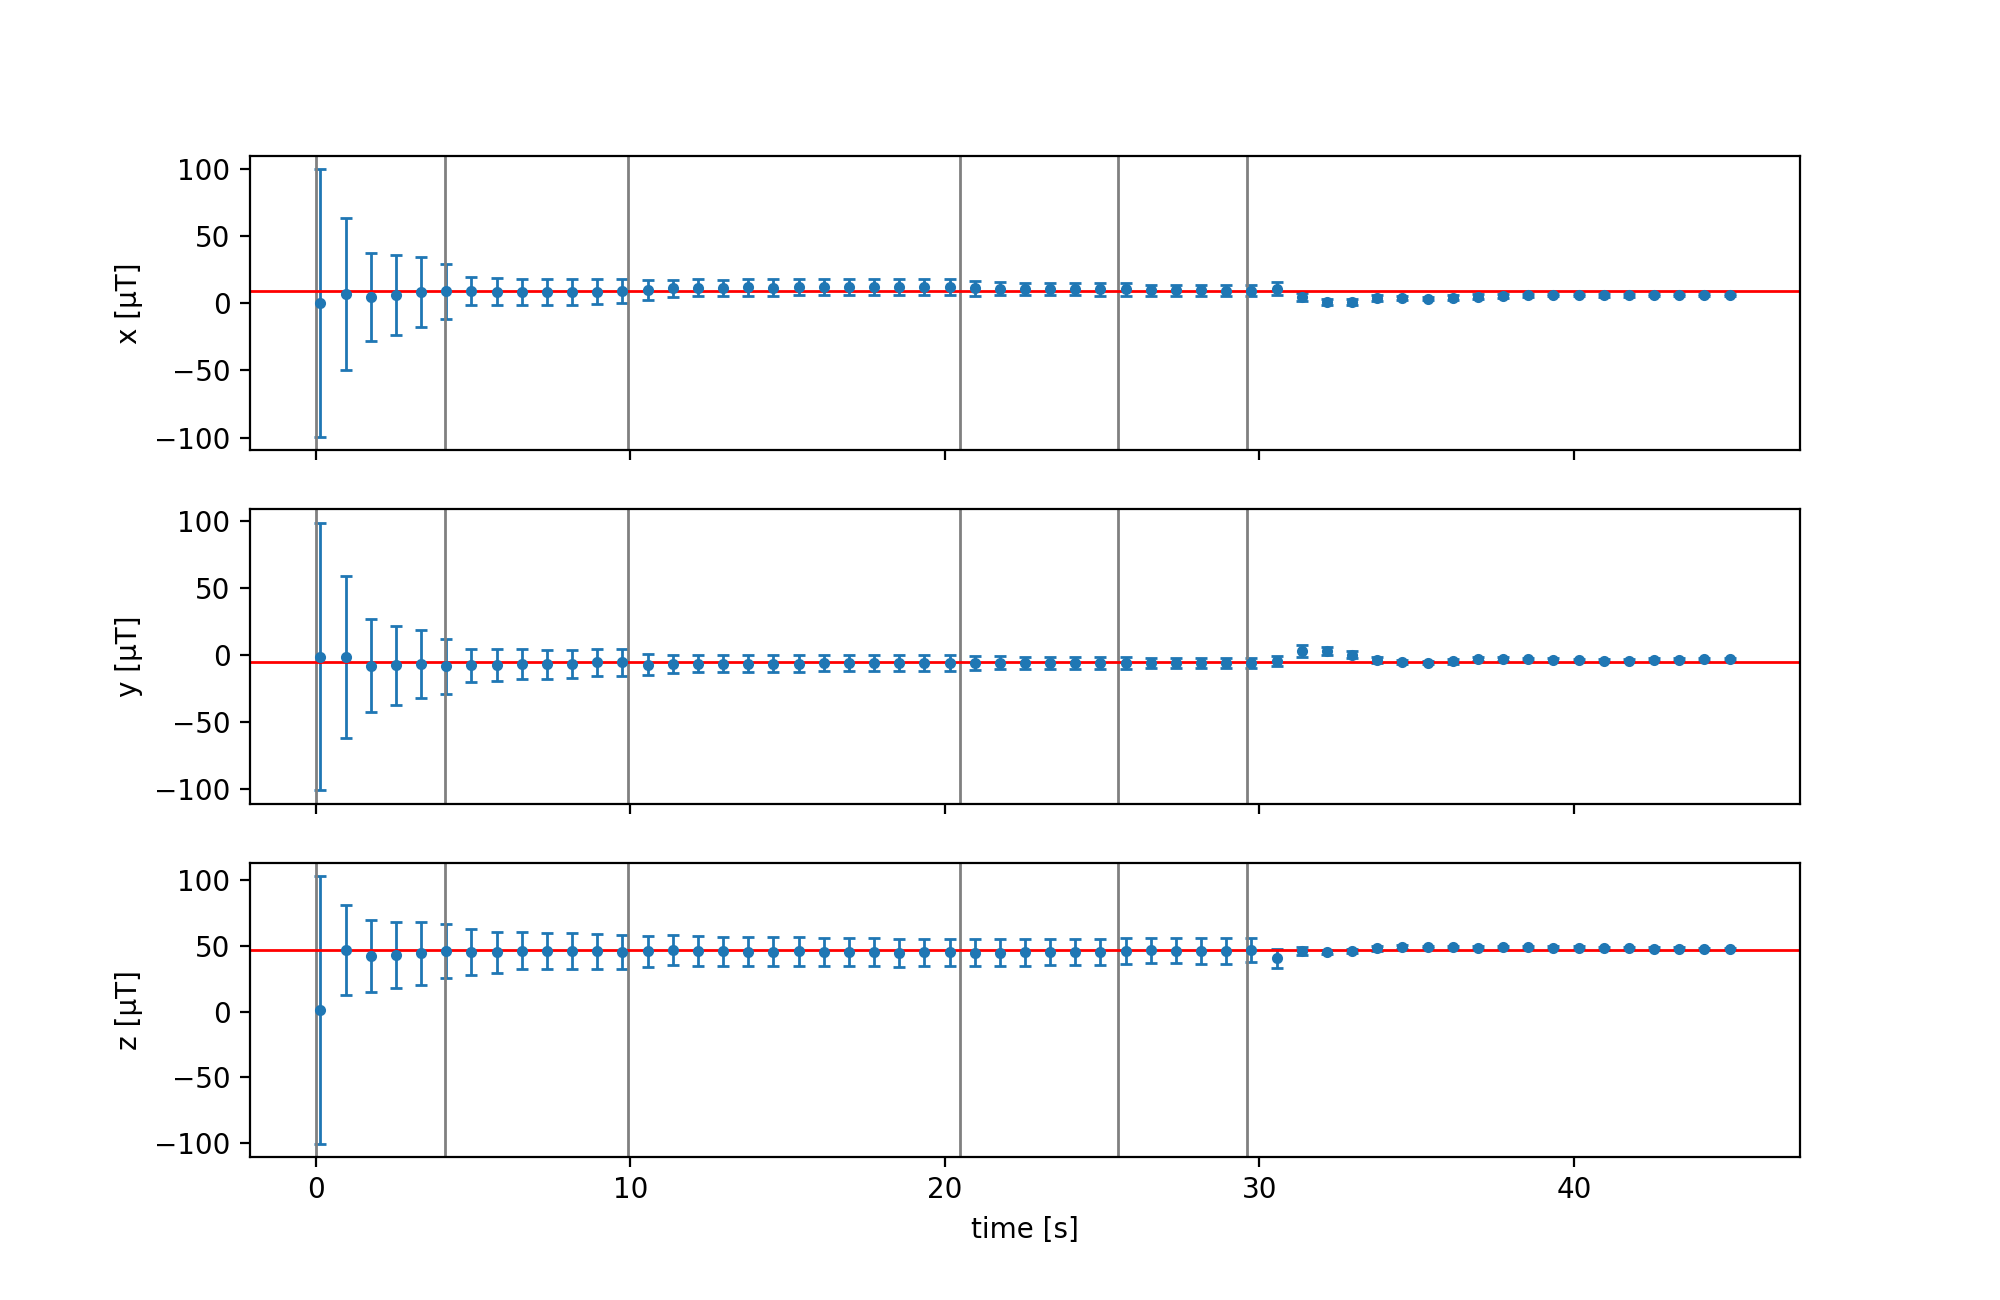
\includegraphics[width=1.0\textwidth]{figures/convergence_nexus5x.png}
    \caption{Estimated hard iron bias and error over time on the LG Nexus 5X.}
    \label{fig:eval_simulation_nexus5x}
\end{figure}

\begin{table}[H]
    \centering
    \resizebox{\columnwidth}{!}{
    \begin{tabular}{ | l | l | r | r | r | r | r | r | r | }
    \hline
    \textbf{Method} & \textbf{Axis} & \textbf{Phase 2.1} & \textbf{Phase 2.2} & \textbf{Phase 2.3} & \textbf{Phase 2.4} & \textbf{Phase 2.5} & \textbf{Phase 2.6} & \textbf{Phase 3} \\ \hline
    PF  & X & $0.4\pm99.4$ & $9.9\pm21.1$ & $7.1\pm9.6$ & $11.6\pm6.1$ & $11.3\pm4.4$ & $10.4\pm4.2$ & $2.9\pm1.1$ \\ \hline
    SYS &   & $-4.4$ & $-4.4$ & $-4.4$ & $-4.4$ & $-4.4$ & $-4.4$ & $10.6$ \\ \hline
    LS  &   & & & & & & & $9.2$ \\ \hline
    PF  & Y & $2.0\pm99.8$ & $-8.8\pm20.9$ & $-5.9\pm10.6$ & $-6.4\pm6.6$ & $-6.7\pm5.1$ & $-6.3\pm4.6$ & $-2.6\pm1.2$ \\ \hline
    SYS &   & $-47.8$ & $-47.8$ & $-47.8$ & $-47.8$ & $-47.8$ & $-47.8$ & $-6.7$ \\ \hline
    LS  &   & & & & & & & $-5.1$ \\ \hline
    PF  & Z & $-1.5\pm100.1$ & $45.9\pm20.7$ & $44.8\pm14.3$ & $40.6\pm10.3$ & $39.2\pm8.2$ & $39.8\pm7.7$ & $48.1\pm1.4$ \\ \hline
    SYS &   & $42.8$ & $42.8$ & $42.8$ & $42.8$ & $42.8$ & $42.8$ & $47.2$ \\ \hline
    LS  &   & & & & & & & $47.0$ \\ \hline
    \end{tabular}
    }
    \caption{Estimated hard iron bias in $\mu T$ with different methods on the LG Nexus 5X.}
    \label{tbl:eval_simulation_nexus5x}
\end{table}

In all our test cases the particle filter was able to converge. The estimated error dropped to approximately $\pm$ 6 $\mu$T after 20 seconds while producing biases of about $\pm$ 10 $\mu$T in the worst case. In phase 3, the accuracy of our filter was worse compared to the \gls{os} and least squares estimates. However, our particle filter produced results when the other methods were not able to. The biases might come from a previous signal processing step like the moving average or the orientation filter. Compared to the earth magnetic field the errors are reasonably small and should not affect the compass too dramatically.

\subsection{Computational performance}

Since we are targeting mobile devices and want to run our particle filter in real-time, the evaluation of the performance is indispensable. A fast algorithm has the benefit of being compatible with older and slower devices and will consume less battery which is a limited resource for mobile devices. Depending on the use case, the performance can be tweaked with the amount of particles. However, reducing the population of the particle filter will also reduce its stability. For a practical use case it is important to find a sweet spot with optimal performance and optimal stability.

The parameter \textsc{minimalRotation} was set to zero in order to measure an upper bound for the \gls{cpu} consumption. Otherwise the parameters were the same as shown in Table \ref{tbl:eval_params}.

The performance measurements are summarized in Table \ref{tbl:eval_performance}. Each value is the result of a 10 second measurement of the CPU time spent in the particle filter divided by real-time passed.

\begin{table}[h]
    \centering
    \begin{tabular}{ | l | r | r | r | r | r | }
    \hline
    \textbf{Device \textbackslash \ Population} & $10^3$ & $10^4$ & $10^5$ \\ \hline
    Google Pixel 3    & 0.00 & 0.06 & 0.51 \\ \hline
    Google Pixel 2    & 0.01 & 0.11 & 0.53  \\ \hline
    Samsung Galaxy S7 & 0.01 & 0.14 & 0.79  \\ \hline
    LG Nexus 5X       & 0.01 & 0.10 & 0.59  \\ \hline
    \end{tabular}
    \caption{CPU time spent in the particle filter divided by real-time passed per device and particle filter population.}
    \label{tbl:eval_performance}
\end{table}
